\documentclass[tikz,border=2pt]{standalone}
\usepackage{amsmath}
\usetikzlibrary{arrows.meta}
\begin{document}
% The system 4a+2b+3c=-5, 2a+3b+4c=2, 3a+4b+5c=6 is typed row by row into A and b;
% solve(A, b) returns (a, b, c) = (-1, 16, -11), and A %*% theta reproduces b.
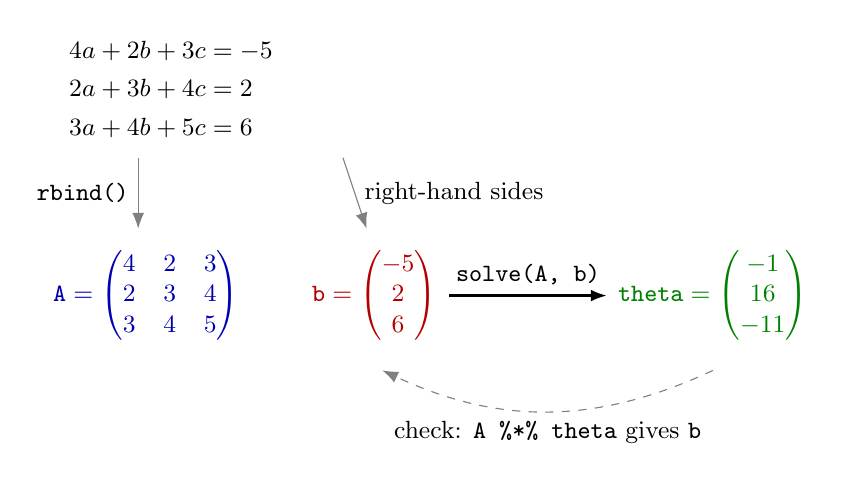
\begin{tikzpicture}[font=\small, >={Latex[length=2mm]}]
  \node[anchor=west] (eq) at (0,0) {$\begin{aligned}4a+2b+3c&=-5\\2a+3b+4c&=2\\3a+4b+5c&=6\end{aligned}$};
  \node[blue!70!black] (A) at (1.1,-2.6) {$\texttt{A}=\begin{pmatrix}4&2&3\\2&3&4\\3&4&5\end{pmatrix}$};
  \node[red!70!black] (b) at (4.0,-2.6) {$\texttt{b}=\begin{pmatrix}-5\\2\\6\end{pmatrix}$};
  \draw[->, gray] (1.0,-0.85) -- node[left, black] {\texttt{rbind()}} (1.0,-1.75);
  \draw[->, gray] (3.6,-0.85) -- node[right, black] {right-hand sides} (3.9,-1.75);
  \node[green!50!black] (th) at (8.3,-2.6) {$\texttt{theta}=\begin{pmatrix}-1\\16\\-11\end{pmatrix}$};
  \draw[->, thick] (4.95,-2.6) -- node[above] {\texttt{solve(A, b)}} (6.95,-2.6);
  \draw[->, dashed, gray] (8.3,-3.55) to[bend left=25] node[below, black] {check: \texttt{A \%*\% theta} gives \texttt{b}} (4.1,-3.55);
\end{tikzpicture}
\end{document}
